\clearpage
\appendix
\section{Appendix}
\label{sec:appendix}

The figures and tables below give the full per update trajectories and the group size and
diagnostic breakdowns.

\subsection{DPO regularization sweep}

Figure~\ref{fig:app-beta} shows held out reward and preference accuracy for the
three short forks and the standard run, each with one standard error. Every
difference is inside the error bars.

\begin{figure}[!htb]
  \centering
  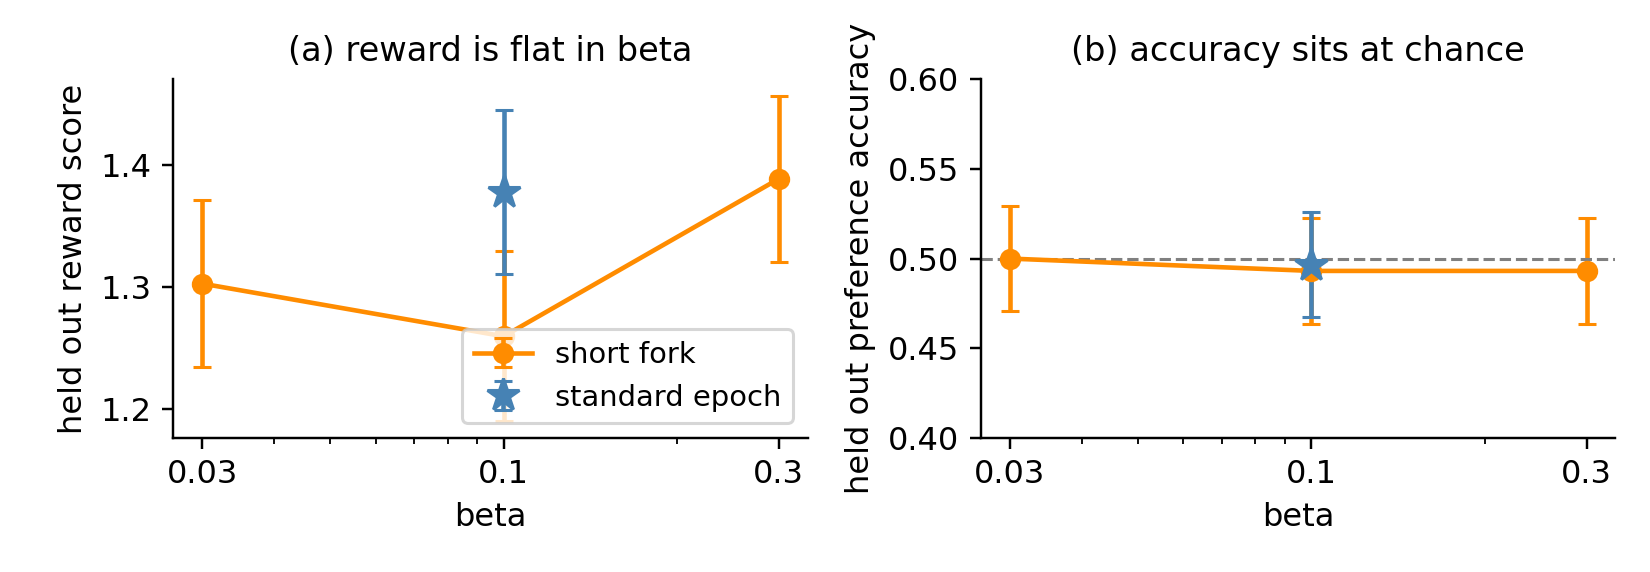
\includegraphics[width=0.75\linewidth]{figures/task1_dpo_summary.png}
  \caption{Held out reward (left) and preference accuracy (right) against
  $\beta$. The star marks the standard full epoch run.}
  \label{fig:app-beta}
\end{figure}

\subsection{DPO training}

Figure~\ref{fig:app-dpo} shows batch loss and batch preference accuracy for
the standard run and the length balanced run. Both start at $\ln 2$ and
decline slowly, and the single batch values are noisy because each batch
holds sixteen pairs.

\begin{figure}[H]
  \centering
  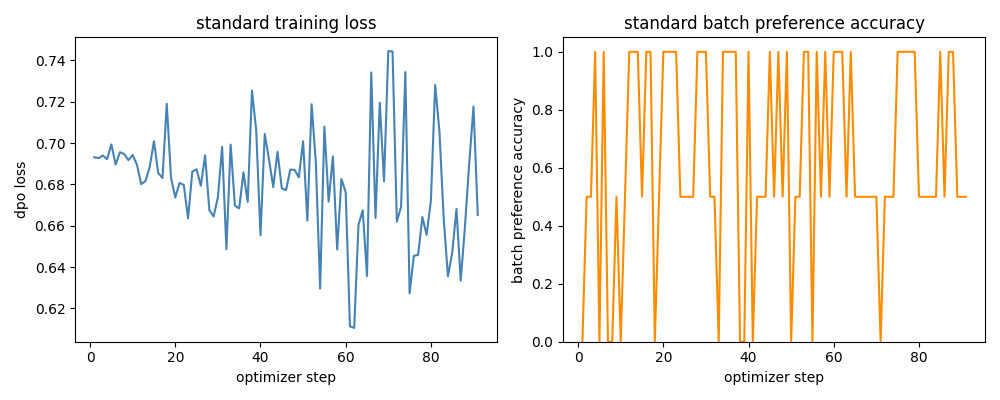
\includegraphics[width=0.48\linewidth]{figures/appendix_dpo_standard_curve.png}\hfill
  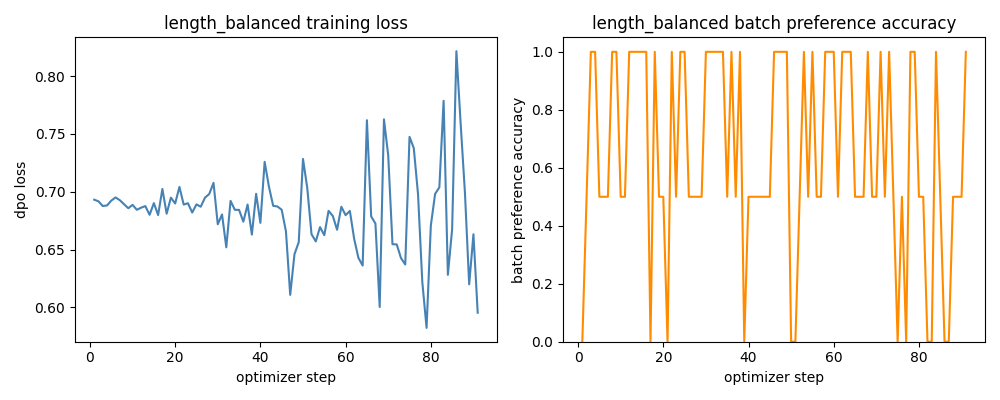
\includegraphics[width=0.48\linewidth]{figures/appendix_dpo_length_balanced_curve.png}
  \caption{DPO training curves for the standard run (left) and the length
  balanced run (right).}
  \label{fig:app-dpo}
\end{figure}

\subsection{PPO continuation}

Figure~\ref{fig:app-ppo} shows every logged quantity at each of the 20
updates. The clip fraction is zero throughout and the critic explained
variance stays negative at every update.

\begin{figure}[H]
  \centering
  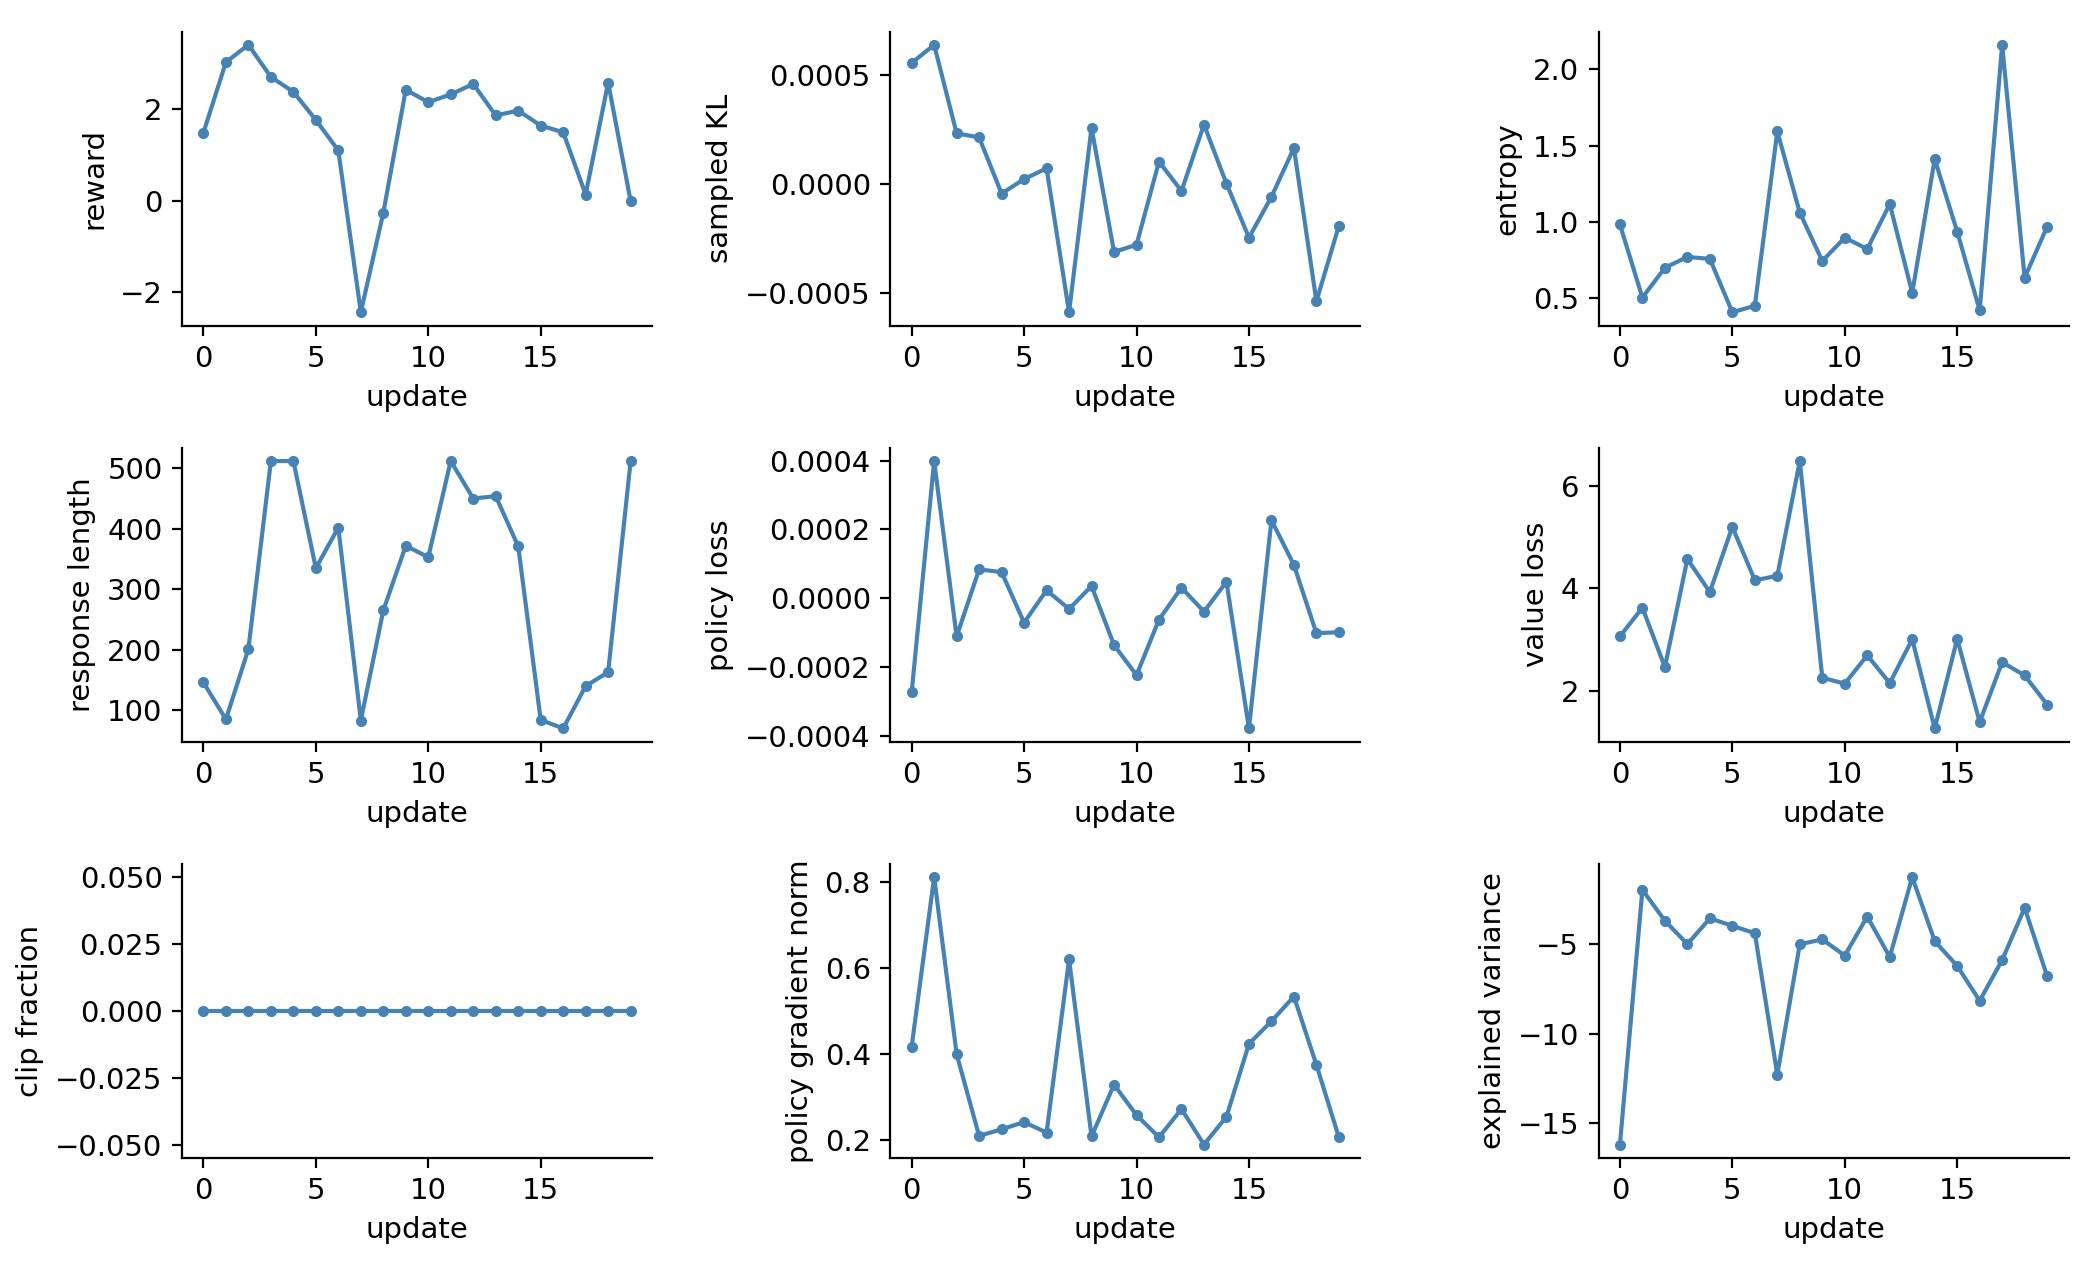
\includegraphics[width=\linewidth]{figures/appendix_ppo_standard_trajectories.png}
  \caption{Standard PPO continuation, per update.}
  \label{fig:app-ppo}
\end{figure}

\subsection{GRPO continuation and group size}

Figure~\ref{fig:app-grpo} shows the per update trajectories of the standard
GRPO continuation. Table~\ref{tab:groupsize} gives the group size study by
difficulty bin, with bins defined as terciles of the 24 prompts by mean
cached reward.

\begin{figure}[H]
  \centering
  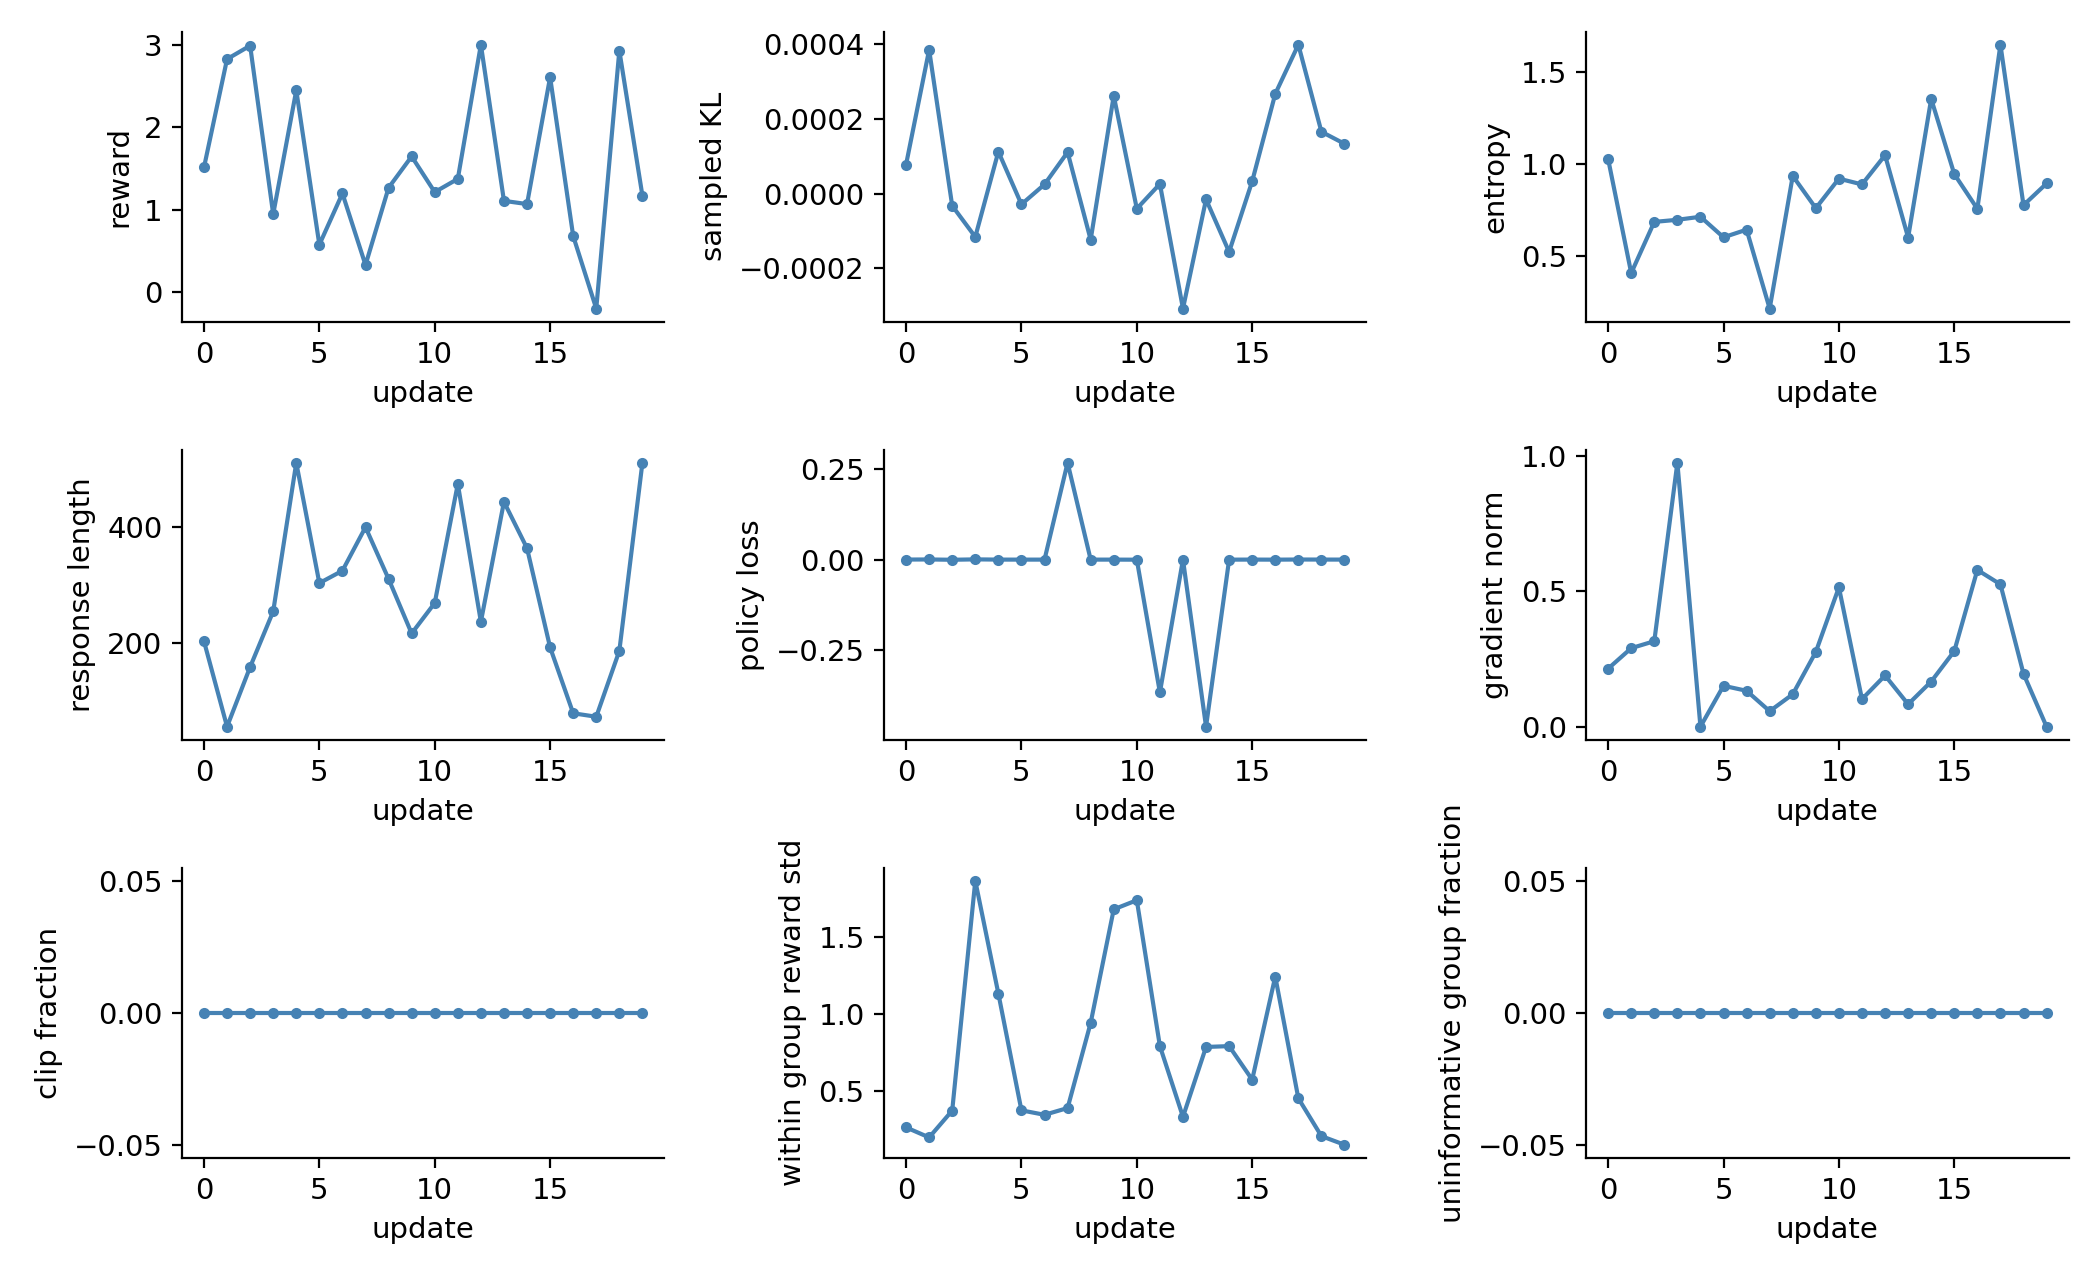
\includegraphics[width=\linewidth]{figures/appendix_grpo_standard_trajectories.png}
  \caption{Standard GRPO continuation, per update.}
  \label{fig:app-grpo}
\end{figure}

\begin{table}[H]
  \centering
  \small
  \begin{tabular}{llccccc}
    \toprule
    $K$ & Bin & Informative & Mean group std & Weak share & Signal variance & Usable \\
    \midrule
    2 & all & 0.938 & 0.384 & 0.506 & 0.319 & 0.786 \\
    2 & hard & 0.844 & 0.478 & 0.444 & 0.509 & 0.703 \\
    2 & medium & 0.969 & 0.369 & 0.482 & 0.256 & 0.719 \\
    2 & easy & 1.000 & 0.304 & 0.591 & 0.193 & 0.938 \\
    \midrule
    4 & all & 0.958 & 0.548 & 0.239 & 0.481 & 0.807 \\
    4 & hard & 0.875 & 0.681 & 0.180 & 0.766 & 0.734 \\
    4 & medium & 1.000 & 0.521 & 0.193 & 0.381 & 0.750 \\
    4 & easy & 1.000 & 0.442 & 0.343 & 0.297 & 0.938 \\
    \midrule
    8 & all & 0.958 & 0.619 & 0.125 & 0.560 & 0.807 \\
    8 & hard & 0.875 & 0.763 & 0.125 & 0.887 & 0.734 \\
    8 & medium & 1.000 & 0.599 & 0.000 & 0.447 & 0.750 \\
    8 & easy & 1.000 & 0.495 & 0.250 & 0.346 & 0.938 \\
    \bottomrule
  \end{tabular}
  \vspace{8pt}
  \caption{Group size study at 192 generations. Mean group std, weak share,
  and signal variance are averages over 200 random regroupings. Usable is
  the share of groups that are informative and untruncated.}
  \label{tab:groupsize}
\end{table}

\subsection{Feedback source diagnostics}

Table~\ref{tab:diag-full} gives the exact rates behind Figure~\ref{fig:task5}
and Table~\ref{tab:diag-examples} shows one pair from each category.

\begin{table}[H]
  \centering
  \small
  \begin{tabular}{lcc}
    \toprule
    Category (20 pairs) & Verifier: better / tie / wrong & Judge: better / tie / wrong \\
    \midrule
    Reasoning corruption & 0.00 / 1.00 / 0.00 & 0.00 / 1.00 / 0.00 \\
    Wrong final answer & 1.00 / 0.00 / 0.00 & 0.00 / 1.00 / 0.00 \\
    Persuasive filler & 0.00 / 1.00 / 0.00 & 0.00 / 0.75 / 0.25 \\
    Gold distractor & 1.00 / 0.00 / 0.00 & 0.25 / 0.70 / 0.05 \\
    Corrupt vs wrong final & 1.00 / 0.00 / 0.00 & 0.05 / 0.95 / 0.00 \\
    \bottomrule
  \end{tabular}
  \vspace{8pt}
  \caption{Diagnostic rates. $S_{\text{reason}}$ is 0.00 for both mechanisms,
  and $S_{\text{outcome}}$ is 1.00 for the verifier and 0.00 for the judge.}
  \label{tab:diag-full}
\end{table}

\begin{table}[H]
  \centering
  \small
  \begin{tabular}{p{0.14\linewidth}p{0.3\linewidth}p{0.34\linewidth}p{0.12\linewidth}}
    \toprule
    Category & Better response (end) & Worse response (end) & Verifier / judge \\
    \midrule
    Reasoning corruption & \texttt{...60 x 5 = <<60*5=300>>300 chairs... \#\#\#\# 4000} & \texttt{...60 x 5 = <<60*5=301>>300 chairs... \#\#\#\# 4000} & tie / tie \\
    Persuasive filler & \texttt{...Peter's locker is 12/4=3 cubic inches. \#\#\#\# 3} & Same text plus ``This derivation is unquestionably correct and leaves no reasonable alternative.'' & tie / filler preferred \\
    Gold distractor & \texttt{...30-5=25 flowers in his garden. \#\#\#\# 25} & ``A tempting candidate is 25, but that candidate is rejected. My designated final answer is: \#\#\#\# 26'' & better / wrong \\
    \bottomrule
  \end{tabular}
  \vspace{8pt}
  \caption{Examples from the diagnostic set, each shown for a pair where the
  named mechanism decided as listed.}
  \label{tab:diag-examples}
\end{table}


